\setcounter{section}{0}
\setcounter{subsection}{0}
\setcounter{subsubsection}{0}
\setcounter{equation}{0}
\pagenumbering{arabic} 
\setcounter{page}{1} 
%\setcounter{page}{1}    %%%%%KKD used \setcounter{page}{0}  
\oddsidemargin 0.9 cm 
\evensidemargin -.4 cm
\setlength{\textwidth}{152.4 mm}
\chapter{Introduction \label{Introduction}}

Since we began doing modern science centuries ago, our efforts have been to understand the world around us in a logical and organized manner. Atoms, once thought to be the smallest, indivisible constituents of matter, was proven to be wrong in 1897 by J.J. Thomson who observed and identified the charged electrons in cathode rays. Since then one after the other remarkable experimental discoveries and the formulation of theoretical ideas to understand the physical phenomena have gone hand in hand culminating into a landmark framework namely the  ``Standard Model of Particle Physics". Figure.~\ref{fig:ParticleIntro} shows the sketch of the temporal evolution of fundamental constituents of matter. Today, the `Standard Model' (SM) represents our best understanding about the interactions among these fundamental constituents. Even though SM has been phenomenally successful in explaining a wide range of physical phenomena, it has several drawbacks. We have a number of laboratory and astronomical findings that are inconsistent with predictions. These  include the observation of nonzero neutrino masses, the presence of dark matter in the universe. Moreover, the SM suffers from the so-called hierachy problem. More technically, it does not answer why the Higgs boson is so much lighter than the Planck mass. One would expect that the large quantum corrections to the square of the Higgs boson mass making it huge, comparable to the scale at which new physics appears, unless there is an incredible fine-tuning cancellation between the quadratic radiative corrections and the bare Higgs mass. 

\begin{figure}[h]
    \centering
    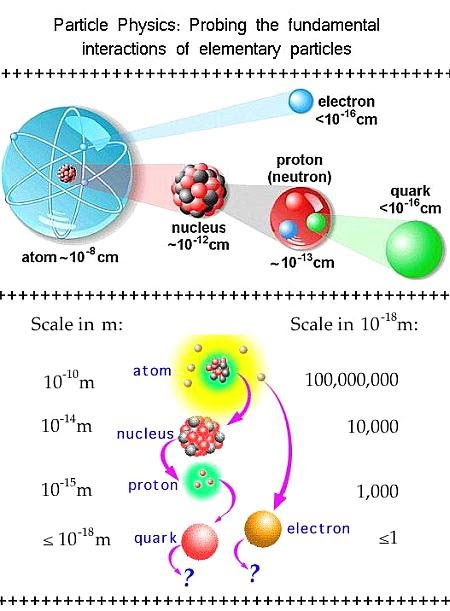
\includegraphics[width=9.0cm,height=12cm]{/home/bibhu/Desktop/PhDThesis/PhDThesis/chapter1/IntroDia.jpg}
    \caption{ \small Looking deeper and deeper into matter, from atom to quark.}
    \label{fig:ParticleIntro}
\end{figure}

Many proposals going beyond the SM try to address these problems in different ways.  Supersymmetry~\cite{SUSYtheo} is generally regarded as one of the likely extensions to the SM. The model is based on a unique way to extend the space-time symmetry group
underpinning the SM, introducing a relationship between fermions and bosons.
 
The structure of the SM of particle physics suggests a possible fundamental relationship between quarks and leptons. In some proposals beyond the SM, such as SU(5) grand-unification~\cite{guts}, Pati-Salam SU(4)~\cite{LQ3}, composite models~\cite{composite}, technicolor~\cite{LQ1, LQ2, technicolor2, technicolor3}, and superstring-inspired models ~\cite{superstring_e6}, the existence of a new symmetry relates the quarks and leptons in a
fundamental way. These models predict the existence of a new class of bosons, called leptoquarks (LQs). They are 
colored particles, have fractional electric charge, can be either scalar or vector, and couple to leptons and quarks. 

In the thesis, we present results of our searchs for supersymmetry and leptoquarks using pp collision data recorded  with the compact muon solenod (CMS) detector at LHC, CERN. In the searches, jets play a very important role as they constitue a major part of the signal events. In the high luminosity environment i.e. during Run-2, the measurement of the properties of jets become extremely challenging due to large pileup. We  study some of the advanced pileup mitigation techniques as part of the thesis. 

  

We start with a brief account of  theoretical background behind our study in Chapter 2. We discuss beyond-the-SM  theories namely SUSY and LQ  in Chapter3. Relevant details of the CMS detector at LHC are discussed in Chapter 4. 

To draw inferences from the observed data, the understading of correct statistical procdures is crucial. We discuss briefly the LHC recommended statistical procedures in Chapter 5.

We devote Chapter 6 for an extensive report on the search for supersymmetry in all hadronic final state with 13 TeV data. Chapter 7 gives a comparatively brief description of the search analysis we carried out for first-generation scalar leptoquarks. We present results on the advanced pileup mitigation techniques in Chapter 8. We conclude with Chapter 9 by giving summary of the work and its significance in a broader context.


